\documentclass[11pt,a4paper]{amsart}
\usepackage[utf8]{inputenc}
\usepackage[T1]{fontenc}
\usepackage{lmodern}
\usepackage{amsmath,amssymb,amsthm}
\usepackage{graphicx}
\usepackage[margin=2.3cm]{geometry}
\usepackage{xcolor}
\usepackage[colorlinks=true,linkcolor=blue!50!black,citecolor=blue!50!black,urlcolor=blue!50!black]{hyperref}

\newtheorem{theorem}{Theorem}
\newtheorem{lemma}[theorem]{Lemma}
\newtheorem{proposition}[theorem]{Proposition}
\newtheorem{corollary}[theorem]{Corollary}
\newtheorem*{propc}{Proposition 2$'$}
\theoremstyle{remark}
\newtheorem*{remark}{Remark}

\newcommand{\eps}{\epsilon}

\title[Sieving intervals and Siegel zeros: a note]{A note on the secondary terms and the prime-gap heuristic in Granville's \texorpdfstring{\lq\lq Sieving intervals and Siegel zeros\rq\rq}{"Sieving intervals and Siegel zeros"}}
\thanks{Code and data are archived at Zenodo, \href{https://doi.org/10.5281/zenodo.24296574}{doi:10.5281/zenodo.24296574};\\ repository: \href{https://github.com/Ruqing1963/granville-2022-siegel-zeros-audit}{github.com/Ruqing1963/granville-2022-siegel-zeros-audit}.}
\author{Ruqing Chen}
\address{GUT Geoservice Inc., Montreal, Canada}
\email{ruqing@hotmail.com}
\date{November 16, 2026}
\subjclass[2020]{11N35, 11M20, 11N05}
\keywords{linear sieve, Siegel zeros, sifting limit, prime gaps}

\begin{document}
\begin{abstract}
We check the quantitative statements near the sifting limit in A.~Granville, \emph{Sieving intervals and
Siegel zeros}, Acta Arith.\ \textbf{205} (2022), 1--19. (i) The last line of the proof of
Proposition~2 replaces $\sqrt{(1-\beta_q)\log q}$ by $\log q/\log y$, although the scale chosen two lines
earlier gives $\log q/(C(u)\log y)$. With the correct substitution the secondary term is
$4y\log q/(\log y)^2$, not $4C(u)y\log q/(\log y)^2$. At the scale $\log y_q=(\log q/(1-\beta_q))^{1/2}$
used in the statement, the proof gives $2(1+C(u)^2)y\log q/(\log y)^2$, which is larger than the printed
term for every $u\in[1,3]$ (by $47\%$ at $u=3$). We state the corrected proposition for every scale.
(ii) In the regime $1-\beta_q\le q^{-\eps}$ the printed constant $2/\eps$ does not follow. The argument
gives $4(1+C(u)^2)/\eps$ at the stated scale, $8/\eps$ at the optimised scale, and at best
$(4+o(1))/\eps$. (iii) In the modified Cram\'er heuristic of Section~4 the parameter $w$ is defined by
$y=(wz)^2$ but used as $y/(\log x)^2$. With $W=y/(\log x)^2$ throughout, the predictions are unchanged.
(iv) The induction proving Theorem~1 applies a relative error term near the boundary of its range, where it
fails. We give an absolute version that is uniform. The first three bullets after Proposition~2, Theorem~1,
and the prime-gap predictions all stand.
\end{abstract}
\maketitle

\section{Introduction}

Granville \cite{G} shows that if there are infinitely many Siegel zeros, then the Jurkat--Richert bounds
for the linear sieve are attained by intervals. He also derives consequences near the sifting limit
$y=z^{2+o(1)}$ (Propositions~1--3), for Jacobsthal's function, and for large gaps between primes. We check
the explicit secondary terms in these statements. We find one slip of substitution in the proof of
Proposition~2, which affects the stated constant and the fourth bullet after it. We also find an
inconsistency between $w$ and $w^2$ in the heuristic of Section~4, and a uniformity issue in the induction
for Theorem~1. None of these affects the qualitative results, and all of them have short repairs.

Page numbers refer to the published version of \cite{G} (pp.~1--19, identical to the Online First pagination). Throughout,
$\delta=\delta_q:=\sqrt{(1-\beta_q)\log q}\to0$, $\log y_q:=(\log q/(1-\beta_q))^{1/2}$, and
$C=C(u)=\bigl(\tfrac12(1-\log^+(u-1))\bigr)^{1/2}$. Note that $C(u)=1/\sqrt2$ on $[1,2]$ and
$C(3)=\sqrt{(1-\log2)/2}=0.3917\ldots$. All identities below were checked symbolically, and all numbers
were recomputed, by a program provided as supplementary material.

\section{Proposition 2: the secondary term}\label{sec:prop2}

Proposition~2 (p.~7) states that for $y=y_q$ and $z=y^{1/u}$ with $u\in[1,3]$ there exist $X$ with
\begin{equation}\label{eq:P2}
S(X,y,z)\ge\frac{2y}{\log y}-(1+o(1))\,\frac{4C(u)\,y\log q}{(\log y)^2}.
\end{equation}
The proof (p.~16) arrives at
\begin{equation}\label{eq:AB}
S(X,y,z)\ge\frac{2y}{\log y}\Bigl(1-\frac1A-\frac{C^2}{B}+O\Bigl(\frac1{A\log q}+\frac1{A^2}+\frac1{B^2}\Bigr)\Bigr),
\qquad A=\frac{\log y}{\log q},\quad B=\frac1{(1-\beta)\log y}.
\end{equation}
We accept \eqref{eq:AB} and only redo the final substitution. Write $\log y=t\log y_q$ with a scale
parameter $t>0$. Then $A=t/\delta$ and $B=1/(t\delta)$, so the relative loss is
\begin{equation}\label{eq:loss}
\frac1A+\frac{C^2}{B}=\delta\Bigl(\frac1t+C^2t\Bigr),\qquad
\frac{2y}{\log y}\Bigl(\frac1A+\frac{C^2}B\Bigr)=2(1+C^2t^2)\,\frac{y\log q}{(\log y)^2},
\end{equation}
where the second form uses $\delta=t\log q/\log y$.

\emph{The stated scale $t=1$.} Here $A=B=1/\delta$ and $1-\beta_q=\log q/(\log y)^2$, so by
\eqref{eq:loss} the secondary term is $2(1+C^2)y\log q/(\log y)^2$. Since $2(1+C^2)-4C=2(1-C)^2>0$, this is
larger than the printed $4C\,y\log q/(\log y)^2$ for every $u$: $3$ against $2\sqrt2=2.828$ on $[1,2]$,
and $2.307$ against $1.567$ at $u=3$. The ratio $(1+C^2)/(2C)$ increases as $C$ decreases, from $1.061$
on $[1,2]$ to $1.472$ at $u=3$.

\emph{The proof's scale $t=1/C$.} The proof chooses $A=C^{-1}\delta^{-1}$ and $B=C\delta^{-1}$, which is
$t=1/C$, the minimiser of $1/t+C^2t$. It then records, correctly, $1-\beta=\log q/(C\log y)^2$ and the
relative loss $2C\delta$. To express this loss as a multiple of $y\log q/(\log y)^2$, one needs $\delta$
in terms of $\log y$. At $t=1/C$ we have $\delta=t\log q/\log y=\log q/(C\log y)$, so $C$ cancels and the
coefficient is $4$. The last line uses instead \lq\lq$\sqrt{(1-\beta)\log q}=\log q/\log y$\rq\rq, which is
the identity at $t=1$. Thus the printed coefficient $4C$ pairs the loss at the scale $t=1/C$ with the
conversion at the scale $t=1$. It is smaller than the coefficient at either scale, since $4C<2(1+C^2)$
and $4C<4$.

\emph{No scale rescues \eqref{eq:P2} for $u>1+\sqrt e$.} By \eqref{eq:loss}, $\kappa(t):=2(1+C^2t^2)>2$
for every $t$. If $C(u)<\frac12$, that is $u>1+\sqrt e=2.649$, then the printed $4C(u)$ is smaller than
$2$, hence smaller than $\kappa(t)$ at every scale (Figure~\ref{fig:main}(a)). For $u<1+\sqrt e$ the
printed value is reached only at $t=\sqrt{2C-1}/C$, and not at the stated $t=1$. As stated,
\eqref{eq:P2} is therefore not proved, and we do not decide whether it is true.

\begin{propc}[corrected form of Proposition 2]
Assume there are infinitely many Siegel zeros, let $u\in[1,3]$, and let $t=t_q>0$ satisfy
$\delta_q=o(t)$ and $t=o(1/\delta_q)$. If $\log y=t\log y_q$ and $z=y^{1/u}$, then there exist $X$ with
\[
S(X,y,z)\ \ge\ \frac{2y}{\log y}\Bigl(1-(1+o(1))\Bigl(\frac1t+C(u)^2t\Bigr)\delta_q\Bigr)
=\frac{2y}{\log y}-(2+o(1))\bigl(1+C(u)^2t^2\bigr)\frac{y\log q}{(\log y)^2}.
\]
In particular, at $t=1$ the coefficient is $2(1+C(u)^2)$. At $t=1/C(u)$, that is for
\[
\log y=C(u)^{-1}\bigl(\log q/(1-\beta_q)\bigr)^{1/2},
\]
we have
\[
S(X,y,z)\ge\frac{2y}{\log y}-(4C(u)+o(1))\sqrt{(1-\beta_q)\log q}\,\frac{y}{\log y}
=\frac{2y}{\log y}-(4+o(1))\frac{y\log q}{(\log y)^2}.
\]
\end{propc}

\begin{proof}
By \eqref{eq:loss} the main loss is $\delta(1/t+C^2t)$. The error terms in \eqref{eq:AB} are
$\delta/(t\log q)$, $\delta^2/t^2$ and $\delta^2t^2$, and the hypotheses on $t$ make each of them
$o(\delta(1/t+C^2t))$. The hypothesis $\delta=o(t)$ also gives $\log y/\log q=t/\delta\to\infty$, which is
the condition $y=q^A$ with $A\to\infty$ used in the proof.
\end{proof}

The first bullet after Proposition~2 has secondary term $(4\delta_0C(u)+o(1))\,y/\log y$ when
$1-\beta_q\le\delta_0^2/\log q$, that is, when $\delta_q\le\delta_0$. This is exactly the first form at
$t=1/C$, so the first bullet is correct at that scale; at the stated scale $y=y_q$ ($t=1$) the
coefficient is $2(1+C(u)^2)\delta_0$. The second and third bullets have unspecified
constants and are unaffected.

\section{The fourth bullet after Proposition 2}\label{sec:bullet4}

The fourth bullet (p.~7) claims
$S(X,y,z)\ge\frac{2y}{\log y}-(2/\eps+o(1))\frac{y\log\log y}{(\log y)^2}$ when $1-\beta_q\le q^{-\eps}$
and $\eps=\eps_q\to0$ slowly. Since $\log\log y=\log t+\frac12\log\log q+\frac12\log\frac1{1-\beta_q}$, we
have $\log\log y\ge\frac\eps2\log q+\frac12\log\log q+\log t$. Hence
$\log q\le(2/\eps+o(1/\eps))\log\log y$ as long as $\log(1/t)=o(\eps\log q)$. Proposition~2$'$
then gives the constant
\[
K(t)=\frac{4(1+C(u)^2t^2)}{\eps},\qquad\text{so}\qquad
\eps K=4(1+C^2)\ (t=1),\quad \eps K=8\ (t=1/C),\quad \eps K\downarrow4\ (t\to0).
\]
Here $4(1+C^2)=6$ on $[1,2]$ and $=6-2\log2=4.614$ at $u=3$. If one inserts the printed coefficient
$4C(u)$ instead, the result is $\eps K=8C(u)\in[3.134,5.657]$. Since $\kappa(t)>2$, we have
$\eps K=2\kappa(t)>4$ at every admissible scale, so $\eps K=2$ is never reached. The infimum $4$ is
approached by $t=1/\log\log q$. This choice is admissible: $\delta_q\le q^{-\eps/2}(\log q)^{1/2}=o(t)$
and $\log(1/t)=\log\log\log q=o(\eps\log q)$, both because $\eps\log q/\log\log q\to\infty$ when
$\eps\to0$ slowly. Hence the fourth bullet holds with $2/\eps$ replaced by $(4+o(1))/\eps$. The printed
$2/\eps$ would need an argument other than \eqref{eq:AB}. The ratio
$\log q/\log\log y_q$ indeed tends to $2/\eps$ from below; for example, $9.67$, $19.82$ and $39.91$ for
$(\eps,\log q)=(0.2,10^3)$, $(0.1,10^4)$ and $(0.05,10^5)$. The comparison with Selberg's
$(\log\log y)^2$ on p.~8 is unaffected.

\begin{figure}[ht]
\centering
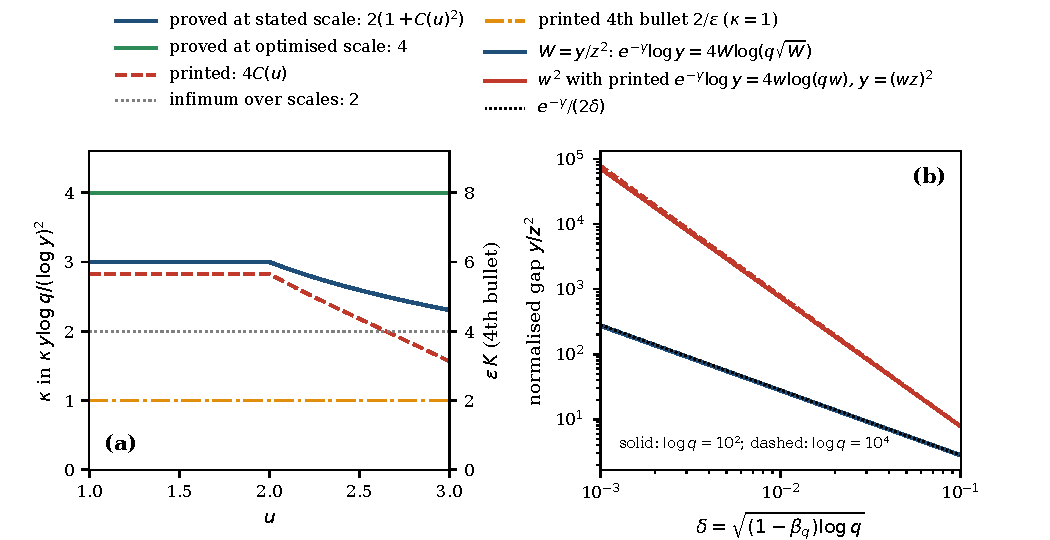
\includegraphics[width=\textwidth]{figures/fig_granville_2022_audit.pdf}
\caption{(a) The coefficient $\kappa$ of $y\log q/(\log y)^2$ in Proposition~2 against $u$. The right
axis shows the corresponding constant $\eps K=2\kappa$ in the fourth bullet. (b) The normalised gap
$y/z^2$ in Section~4 against $\delta$, for $z=\log x$. Blue: the consistent relation for $W=y/z^2$. Red: $w^2$, where $w$
solves the printed relation and $y=(wz)^2$. The blue curves coincide with Granville's $w$ to within
$3\%$.}\label{fig:main}
\end{figure}

\section{Section 4: \texorpdfstring{$w$}{w} against \texorpdfstring{$w^2$}{w squared}}\label{sec:gap}

On p.~17 Granville applies Proposition~3 with $\log y=2(\log q/(1-\beta))^{1/2}$. Then
$(1-\beta)y=4y\log q/(\log y)^2$, and he puts $y=(wz)^2$ to get
\[
S(X,y,z)\lesssim\frac{8y}{(\log y)^2}\log(qw),
\]
which is correct because $\log(qw^2)+\log q=2\log(qw)$. The comparison on p.~18 with the heuristic of \cite{GL},
$\min_XS\sim2e^{-\gamma}(\log x)^2/\log y$, where $z\asymp\log x$, gives
\[
e^{-\gamma}\log y\ \lesssim\ 4\,W\log(qw),\qquad W:=\frac{y}{(\log x)^2},
\]
not $e^{-\gamma}\log y\lesssim4w\log(qw)$ as printed. In the subsequent predictions the bound for $w$ is
read as a bound for $(p_{n+1}-p_n)/(\log p_n)^2\asymp W$. That is the right reading for $W$, but not for
$w$: if $z=c\log x$ then $W=c^2w^2$ (so $W=y/z^2=w^2$ for $c=1$, as in Figure~\ref{fig:main}(b)), and
$\log(qw)=\log(q\sqrt W)+O(1)$. The clean version uses $W$ throughout:
\begin{gather*}
S(X,y,z)\lesssim\frac{8y}{(\log y)^2}\log\bigl(q\sqrt W\bigr),\qquad
e^{-\gamma}\log y\lesssim4W\log\bigl(q\sqrt W\bigr),\\
W\gtrsim\frac{e^{-\gamma}\log y}{4\log q}=\frac{e^{-\gamma}/2}{\sqrt{(1-\beta)\log q}}.
\end{gather*}
This is the bound printed for $w$, now for the correct quantity. All predictions on p.~18 then follow as
stated. For example, $1-\beta\asymp(\log q)^{-\kappa}$ gives
$1/\delta\asymp(\log\log p_n)^{1-2/(\kappa+1)}$. Figure~\ref{fig:main}(b) shows $W$ and $w^2$: the literal
reading $y=(wz)^2$ with the printed $w$ would square the predicted normalised gap.

\section{Theorem 1: uniformity in the induction}\label{sec:thm1}

Theorem~1 (p.~10) asserts
$\pi_k(x,z;q,a)=(1+(-1)^k\chi(a)+O(\varDelta))\,\pi_{k,q}(x,z)/\phi(q)$ for fixed $u>1$ and $x=z^u$.
It needs no extra hypothesis $k<u$, because for $k\ge u$ both sides vanish. The induction, however,
applies the case $k-1$ to $x'=x/p$ with $z<p\le x/z^{k-1}$. So $\log x'/\log z$ ranges over
$(k-1,u-1]$ and is not fixed, and near $x'=z^{k-1}$ the relative error is not available. For $k-1=1$,
Corollary~4 gives $\pi_1(x',z;q,b)=\pi(x';q,b)-\pi(z;q,b)$ with error $O(\varDelta\pi(x')/\phi(q))$,
while $\pi_{1,q}(x',z)=\pi(x')-\pi(z)\to0$ relative to $\pi(x')$ as $x'\to z^+$. For $z=2000$, the ratio
$\pi(x')/(\pi(x')-\pi(z))$ is $2.07$, $14.8$ and $51.5$ at $x'=z^{1.1},z^{1.01},z^{1.003}$. The remedy is
to carry an absolute error.

\begin{lemma}\label{lem:abs}
Under the hypotheses of Theorem~1, for every $k\ge1$ and $U\ge1$, uniformly for $z\ge q^A$,
$z^k\le x\le z^U$ with $\varDelta_\beta(x)\le\varDelta$, and $(a,q)=1$,
\[
\pi_k(x,z;q,a)=\bigl(1+(-1)^k\chi(a)\bigr)\frac{\pi_{k,q}(x,z)}{\phi(q)}+O_{k,U}\Bigl(\varDelta\,\frac{x}{\phi(q)\log z}\Bigr).
\]
\end{lemma}

\begin{proof}[Sketch]
\emph{The case $k=1$.} Since $z\ge q^A>q$, no prime in $(z,x]$ divides $q$, so
$\pi_1(x,z;q,a)=\pi(x;q,a)-\pi(z;q,a)$. Apply (8) at $x$ and at $z$; both are $\ge q^A$, and
$\varDelta_\beta(z)\le\varDelta_\beta(x)\le\varDelta$. This gives the main term
$(1-\chi(a))(\pi(x)-\pi(z))/\phi(q)$ with error $O(\varDelta\,\pi(x)/\phi(q))$, and $\pi(x)\ll x/\log z$.

\emph{The step $k-1\to k$.} As on p.~10,
\[
\pi_k(x,z;q,a)=\frac1k\sum_{z<p\le x/z^{k-1}}\pi_{k-1}(x/p,z;q,a/p)+O\Bigl(\frac{x}{\phi(q)z\log z}\Bigr),
\]
and likewise $\frac1k\sum_p\pi_{k-1,q}(x/p,z)=\pi_{k,q}(x,z)+O(x/(z\log z))$. Each $x/p$ lies in
$[z^{k-1},z^{U-1}]$, so the case $k-1$ applies to every term, \emph{including those with $x/p$ close to
$z^{k-1}$}. The reason is that its error term $O(\varDelta\,(x/p)/(\phi(q)\log z))$ does not involve
$\pi_{k-1,q}(x/p,z)$. Since $\sum_{z<p\le x}1/p\le\log U+O(1)$, these errors add up to
\[
\sum_{z<p\le x/z^{k-1}}\frac{\varDelta\,x/p}{\phi(q)\log z}\ll\frac{\varDelta\,x\log U}{\phi(q)\log z}.
\]
In the main terms, $\chi(a/p)=\chi(a)\chi(p)$. When $\chi(p)=-1$ the factor $1+(-1)^{k-1}\chi(a/p)$
equals $1+(-1)^k\chi(a)$. The primes with $\chi(p)=1$ change it by at most $2$, and they contribute
$\ll\sum_{\chi(p)=1,\,z<p\le x}x/(p\,\phi(q)\log z)$, using $\pi_{k-1,q}(t,z)\ll_{k,U}t/\log z$. By (8),
$\#\{p\le t:\chi(p)=1\}\ll\varDelta\,\pi(t)$ for $t\ge q^A$, and partial summation bounds this
contribution by $\ll\varDelta\,x(1+\log U)/(\phi(q)\log z)$, as on p.~11. Finally,
$x/(\phi(q)z\log z)\ll\varDelta\,x/(\phi(q)\log z)$, because $1/z\le q^{-A}\ll1-\beta\le\varDelta$ by
Siegel's theorem.
\end{proof}

For fixed $u>k$, (9) gives $\pi_{k,q}(z^u,z)\asymp_{k,u}x/\log z$, so Lemma~\ref{lem:abs} implies
Theorem~1 as stated. The boundary terms are in fact harmless even in the original argument. Their total
is $\ll\varDelta\sum_{z<p\le x/z}\pi(z)/\phi(q)\ll\varDelta x/(\phi(q)\log z\,\log(x/z))$; for example, at
$z=2000$ and $u=2.2$ the sum is $0.10\,x/\log z$. The conclusions of Theorem~1 and Corollary~5 stand.

\begin{thebibliography}{9}
\bibitem{G} A.~Granville, \emph{Sieving intervals and Siegel zeros}, Acta Arith.\ \textbf{205} (2022),
no.~1, 1--19, \href{https://doi.org/10.4064/aa201002-25-6}{doi:10.4064/aa201002-25-6}; arXiv:2010.01211.
\bibitem{GL} A.~Granville and A.~Lumley, \emph{Primes in short intervals: heuristics and calculations},
Exp.\ Math.\ \textbf{32} (2023), no.~2, 378--404, \href{https://doi.org/10.1080/10586458.2021.1927256}{doi:10.1080/10586458.2021.1927256}.
\end{thebibliography}
\end{document}
